\subsection{Berechnung der Suszeptibilität}
Die magnetische Flussdichte $\vec{B}$ setzt sich aus der magnetischen Feldstärke
$\vec{H}$, der Induktionskonstanten $\mu_0$ und der Magnetisierung $\vec{M}$
zusammen:
\begin{equation}
  \vec{B} = \mu_0 \vec{H} + \vec{M}.
\end{equation}
Die Magnetisierung $\vec{M}$ entsteht durch atomare magnetische Momente in der
Substanz und ist von der magnetischen Feldstärke $\vec{H}$ abhänging:
\begin{equation}
  \vec{M} = \mu_0 \chi \vec{H}.
\end{equation}
Die Suszeptibilität $\chi$ hängt von $\vec{H}$ und der Temperatur $T$ ab.
Magnetische Momente können einen Diemagnetismus und einen Paramagnetismus
hervorrufen. Die Diamagnetismus tritt bei allen Atomen auf, er beruht auf einer
Induktion magnetischer Momente durch ein von außen angelegtes Magnetfeld.
Da die Induktion dem von außen angelegten Magnetfeld entgegenwirkt ist $\chi$
beim Diamagnetismus kleiner als 0. Der Paramagnetismus wird nur beobachtet, wenn
der Drehimpuls nicht verschwindet. Er ensteht durch die Orientierung der
magnetischen Momente, welche mit dem Drehimpuls gekoppelt sind, relativ zu einem
äußeren Magnetfeld. Im Gegensatz zum Diamagnetismus ist der Paramagnetismus somit
temperaturabhänging, da die thermische Bewegung die Ausrichtung stört. Beim
Paramagnetismus ist $\chi$ größer als 0.

Der Gesamtdrehimpuls $\vec{J}$ eines Atoms setzt sich aus dem Bahndrehimpuls $\vec{L}$
der Elektronenhülle, dem Eigendrehimpuls (Spin) $\vec{S}$ der Elektronen und dem
Kerndrehimpuls zusammen:
\begin{equation}
  \vec{J} = \vec{L} + \vec{S}
\end{equation}
, mit $\vec{L} = \sum \vec{\ell_\su{i}}$ und $\vec{S} = \sum \vec{s_\su{i}}$.
Der Kerndrehimpuls wird hier nicht weiter betrachtet,
da er sich nur in sehr starken äußeren Magnetfeldern bemerkbar macht.

Aus der Quantenmechanik folgt:
\begin{align}
  \vec{\mu_\su{L}} &= -\frac{\mu_\su{B}}{\hbar} \vec{L} \\
  \vec{\mu_\su{S}} &= -g_\su{S}\frac{\mu_\su{B}}{\hbar} \vec{S}
\end{align}
mit dem Bohrschen Magneton $\mu_\su{B} = \frac{e \hbar}{2m_0}$ und dem
gyromagnetischen Verhältnis $g_\su{S}$ des freien Elektrons. $e$ und $m_0$
beschreiben Ladung bzw. Ruhemasse des Elektrons.

Für die Beträge aller drei Drehimpulse gilt analog
\begin{equation}
  |\vec{J}| = \sqrt{J(J+1)} \hbar.
\end{equation}
Damit ergibt sich:
\begin{align}
  |\vec{\mu_\su{L}}| &= \mu_\su{B}\sqrt{L(L+1)} \\
  |\vec{\mu_\su{S}}| &= g_\su{S}\mu_\su{B}\sqrt{S(S+1)}.
\end{align}
Mit Abbildung \ref{fig:drehimpuls} ergibt sich die Beziehung
\begin{equation}
  |\vec{\mu_\su{J}}| = |\vec{\mu_\su{S}}| \cos{(\alpha)} + |\vec{\mu_\su{L}}|
  \cos{(\beta)}.
\end{equation}
\begin{figure}
  \centering
  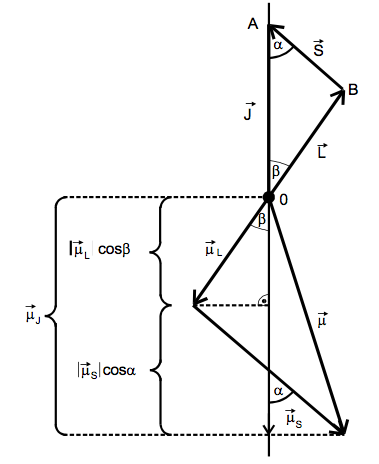
\includegraphics[width=6cm]{bilder/drehimpuls.png}
  \caption{Vektordiagramm der Drehimpulsvektoren einer Elektronenhülle und ihren
  magnetischen Momenten \cite{606}}
  \label{fig:drehimpuls}
\end{figure}
Mit der Annahme $g_\su{S} = 2$ folgt der Ausdruck
\begin{equation}
  |\vec{\mu_\su{J}}| = \mu_\su{B} \sqrt{J(J+1)} \frac{3J(J+1)+\Big(S(S+1)
  -L(L+1)\Big)}{2J(J+1)}.
\end{equation}
Dabei wird
\begin{equation}
  g_\su{J} = \frac{3J(J+1)+\Big(S(S+1) -L(L+1)\Big)}{2J(J+1)}
\end{equation}
als Landé-Faktor bezeichnet.
Es folgt vereinfacht:
\begin{equation}
  |\vec{\mu_\su{J}}| = \mu_\su{B} g_\su{J} \sqrt{J(J+1)}.
\end{equation}
Ein weiteres Phänomen ist die Richtungsquantelung. Sie besagt, dass nur die Winkel,
zwischen der Richtung des äußeren Magnetfeldes und der Lage von $\vec{\mu_\su{J}}$,
möglich sind, bei denen die z-Komponente von $\vec{\mu_\su{J}}$ in Feldrichtung
ein ganzzahliges Vielfaches von $\mu_\su{B}g_\su{J}$ ist, also
\begin{equation}
  \mu_\su{J_\su{z}} = -\mu_\su{B}g_\su{J}\cdot m. \label{eqn:ori}
\end{equation}
$m$ ist die ganzzahlige Orientierungsquantezahl. Es gibt genau $2J+1$
Einstellmöglichkeiten. Zu jeder dieser Einstellmöglichkeit gehört auch eine
potentielle Energie. Die Aufspaltung eines Energieniveaus in $2J+1$ Unterniveaus
beim Anlegen eines Feldes wird als Zeeman-Effekt bezeichnet.
Nun kann die Magnetisierung mit \eqref{eqn:ori} berechnent werden. Dazu werden
die Häufigkeiten mit denen ein gewisse Orientierung auftritt mit den dazugehörigen
Beträgen multipliziert und dann aufsummiert. Nach mehreren Umformungen ergibt
sich für die paramagnetische Suszeptibilität:
\begin{equation}
  \chi = \frac{\mu_0 \mu_\su{B}^2 g_\su{J}^2 N J(J+1)}{3kT}
\end{equation}
, mit $N$ als Anzahl der Momente pro Volumeneinheit, $k$ der Boltzmann-Konstanten
 und $T$ der Temperatur. Somit ist $/chi \propto \sfrac{1}{T}$. Dies wird als Curiesches
 Gesetz des Paramagnetismus bezeichnet.

 Besonders gut lässt sich der Paramagnetismus bei Seltenerdmetallen beobachten,
 da diese große Drehimpulse besitzen, welche von inneren Elektronen erzeugt werden,
 hauptsächlich von denen der 4f-Schale. Die Hundschen Regeln legen dabei die
 Anordnung und den Gesamtdrehimpuls $\vec{J}$ fest.
 \begin{itemize}
   \item $\vec{S} = \sum \vec{s_\su{i}}$ unter Berücksichtigung des
   Pauli-Prinzips \\
   \item Der maximale Drehimpuls $\vec{L} = \sum \vec{\ell_\su{i}}$ entsteht \\
   \item $\vec{J} = \vec{L}-\vec{S}$, wenn die Schale weniger als halb,
   $\vec{J}= \vec{L}+\vec{S}$, wenn die Schale mehr als halb gefüllt ist \\
 \end{itemize}
